% Run upc2026-wp3-v1; selection-results.json; blind-results.json; metrics.csv; blind-conditional.csv; models B0/B2; scenario nominal_gaussian_10mm.

\section{Validation and model choice}\label{sec:validation}

\subsection{Design and sealing}

The development, selection, and blind sets contained 84, 260, and 520 distinct synthetic shots, respectively. The nominal forecast used the two noisy frame centres with independent 10\,mm Gaussian errors in each coordinate. The generation model used an independent third-order Runge--Kutta implementation with step halving. An event search refined first plane and turf crossings under the same geometric and time-tie rules as the forecast. We retained separate strata for matched trajectories, wind, speed-dependent drag, time-varying transverse force, sensor error, and combined stress. The enriched challenge set probed lateral misses, shallow launches, and nearly vertical launches. It was excluded from the equal-weight mean across the six core strata. The supplied kick was outside the benchmark.

We locked each prediction CSV before revealing the corresponding labels. The selection lock contained all six model families. The blind lock used the chosen pair with the same per-model settings. A forecast received only the two observed frame centres, their times, and the nominal scenario. The scorer joined the predictions to the held-out truth and scoring strata by case ID.

\subsection{Scoring and selection}

The primary outcome was centre entry. The Brier loss was $(p-I)^2$, where $I$ is the truth indicator. A forecast with resolved event mass $p$ and failed mass $f$ received the worse loss at the endpoints $p$ and $p+f$. Entirely invalid or missing forecasts received unit loss. We also report ordinary Brier loss for exact probabilities and score plane arrival, radius clearance, and first turf contact separately. A point abstention does not remove a valid event probability. In conditional crossing scores, the location uses resolved plane draws and truth that reached the plane.

An aerodynamic model needed a reduction of at least 0.01 in the equal-core-stratum penalized entry loss and a gain greater than one paired bootstrap standard error. It could lose at most 0.02 in each core stratum, produce at most 1.0\% entirely invalid forecasts, and fall no more than 5 percentage points below nominal 95\% coverage. Region coverage uses highest-mass square cells of side 0.10\,m with all ties at the cutoff included. A conditional region requires at least 100 effective draws. The paired bootstrap draws 2,000 resamples of physical shots within strata.

\subsection{Locked results}

Selection retained B0, with B2 as the locked comparator. Their selection penalized entry losses were 0.0571 and 0.1529. No aerodynamic candidate passed the registered selection gates. The blind comparison is therefore descriptive. The blind equal-core-stratum losses were 0.0721 and 0.1732. The gain, defined as comparator loss minus selected loss, was 0.1010, with paired 95\% interval 0.0753 to 0.1304. The blind comparison does not support a confirmed aerodynamic upgrade.

The empirical coverage of nominal 95\% core regions was 7.1\% for B0 (31/437 supported regions among 440 true plane crossings) and 62.7\% for B2 (271/432 supported regions among 440 true plane crossings). The nominal locations substantially undercovered in this benchmark. The selected model's lower entry loss supports its use as a reference event forecast under the tested assumptions. Its nominal location regions have much weaker calibration.

\begin{table}[htbp]
\centering
\renewcommand{\thetable}{T3}
\caption{Locked blind evaluation by stratum. Eligible truth excludes truth-solver failures. The penalized entry score uses all eligible cases. The ordinary score gives the exact-probability denominator in parentheses. Forecast failures are shown as any unresolved or invalid forecast versus entirely invalid. Abstentions are counted among resolved forecasts. Coverage uses the supported regions among true plane crossings. Energy scores condition on plane crossing, with the scored count in parentheses.}
\label{tab:validation}\label{tab:T3}
\resizebox{\linewidth}{!}{%
\begin{tabular}{llrrrrrrrr}
\hline
Stratum & Model & Truth eligible/total & Penalized Brier & Ordinary Brier ($n$) & Failures any/full & Abstentions/resolved & Regions/truth plane & 95\% coverage & Energy, m ($n$) \\
\hline
Matched & B0 & 80/80 & 0.0885 & 0.0885 (80) & 0/0 & 40/80 & 70/71 & 4.3\% & 0.3284 (70) \\
Matched & B2 & 80/80 & 0.1500 & 0.1519 (79) & 1/0 & 20/80 & 71/71 & 69.0\% & 0.6629 (71) \\
Wind & B0 & 80/80 & 0.0661 & 0.0661 (80) & 0/0 & 45/80 & 75/75 & 10.7\% & 0.3205 (75) \\
Wind & B2 & 80/80 & 0.1557 & 0.1506 (78) & 2/0 & 20/80 & 75/75 & 78.7\% & 0.5220 (75) \\
Drag & B0 & 80/80 & 0.0554 & 0.0554 (80) & 0/0 & 47/80 & 72/72 & 5.6\% & 0.3322 (72) \\
Drag & B2 & 80/80 & 0.1414 & 0.1442 (78) & 2/0 & 35/80 & 72/72 & 76.4\% & 0.5182 (72) \\
Lift & B0 & 80/80 & 0.0437 & 0.0437 (80) & 0/0 & 37/80 & 74/74 & 2.7\% & 0.3225 (74) \\
Lift & B2 & 80/80 & 0.1445 & 0.1445 (80) & 0/0 & 23/80 & 73/74 & 63.0\% & 0.6800 (73) \\
Sensor & B0 & 80/80 & 0.0869 & 0.0880 (79) & 1/0 & 46/80 & 73/75 & 8.2\% & 0.3237 (73) \\
Sensor & B2 & 80/80 & 0.2446 & 0.2410 (77) & 3/0 & 32/80 & 71/75 & 45.1\% & 1.1001 (71) \\
Combined & B0 & 80/80 & 0.0921 & 0.0921 (80) & 0/0 & 37/80 & 73/73 & 11.0\% & 0.3675 (73) \\
Combined & B2 & 80/80 & 0.2028 & 0.2028 (80) & 0/0 & 29/80 & 70/73 & 42.9\% & 0.9034 (70) \\
Challenge & B0 & 40/40 & 0.0010 & 0.0010 (40) & 0/0 & 32/40 & 22/22 & 0.0\% & 0.4236 (22) \\
Challenge & B2 & 40/40 & 0.0237 & 0.0268 (35) & 5/0 & 30/40 & 22/22 & 68.2\% & 0.9297 (22) \\
\hline
\end{tabular}}
\end{table}

Figure~\ref{fig:F5} shows event reliability and the frequency of numerical failures and point abstentions. Matched, pooled single-factor stress, combined stress, and challenge are shown separately. Figure~\ref{fig:F6} reports joint coverage at nominal 50\%, 80\%, and 95\%, with crossing error on the common valid cases. Sparse reliability bins and unsupported comparisons are marked in the figure evidence.

\begin{figure}[htbp]
\centering
\renewcommand{\thefigure}{F5}
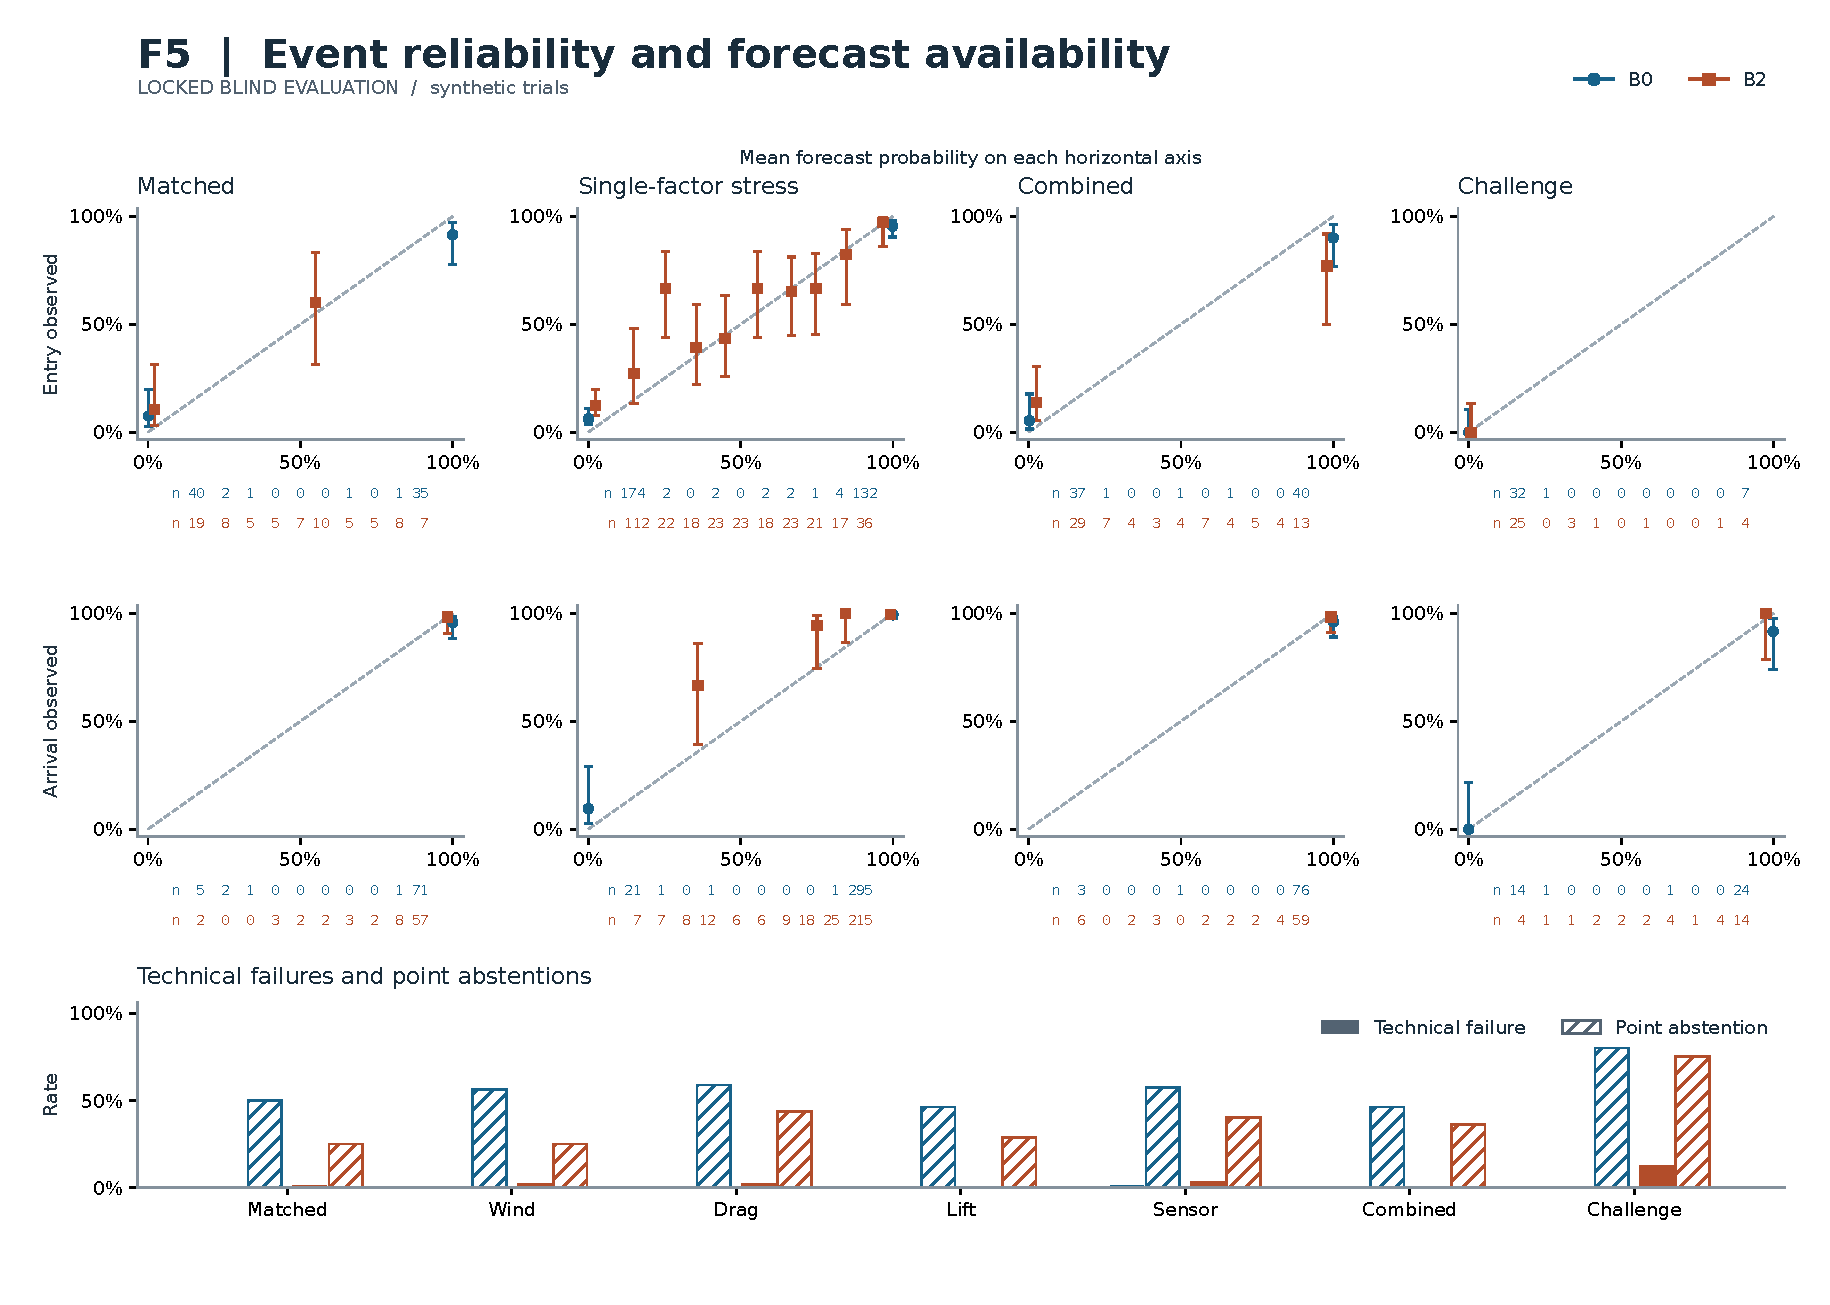
\includegraphics[width=\linewidth]{figures/F5.pdf}
\caption{Calibration of exact probabilities for centre entry and forward plane arrival on synthetic trials with resolved truth. Nominal decile bins include 1 in the final bin. Numbers below each panel are per-bin counts in model order. Bins below the locked minimum are omitted from the curves. Vertical bars are 95\% Wilson intervals. The single-factor panels pool wind, drag, lift and sensor stress. Technical failures use all cases with resolved truth. Point abstentions use cases with a resolved forecast and a recorded point decision. The challenge sample is reported separately.}
\label{fig:F5}
\end{figure}

\begin{figure}[htbp]
\centering
\renewcommand{\thefigure}{F6}
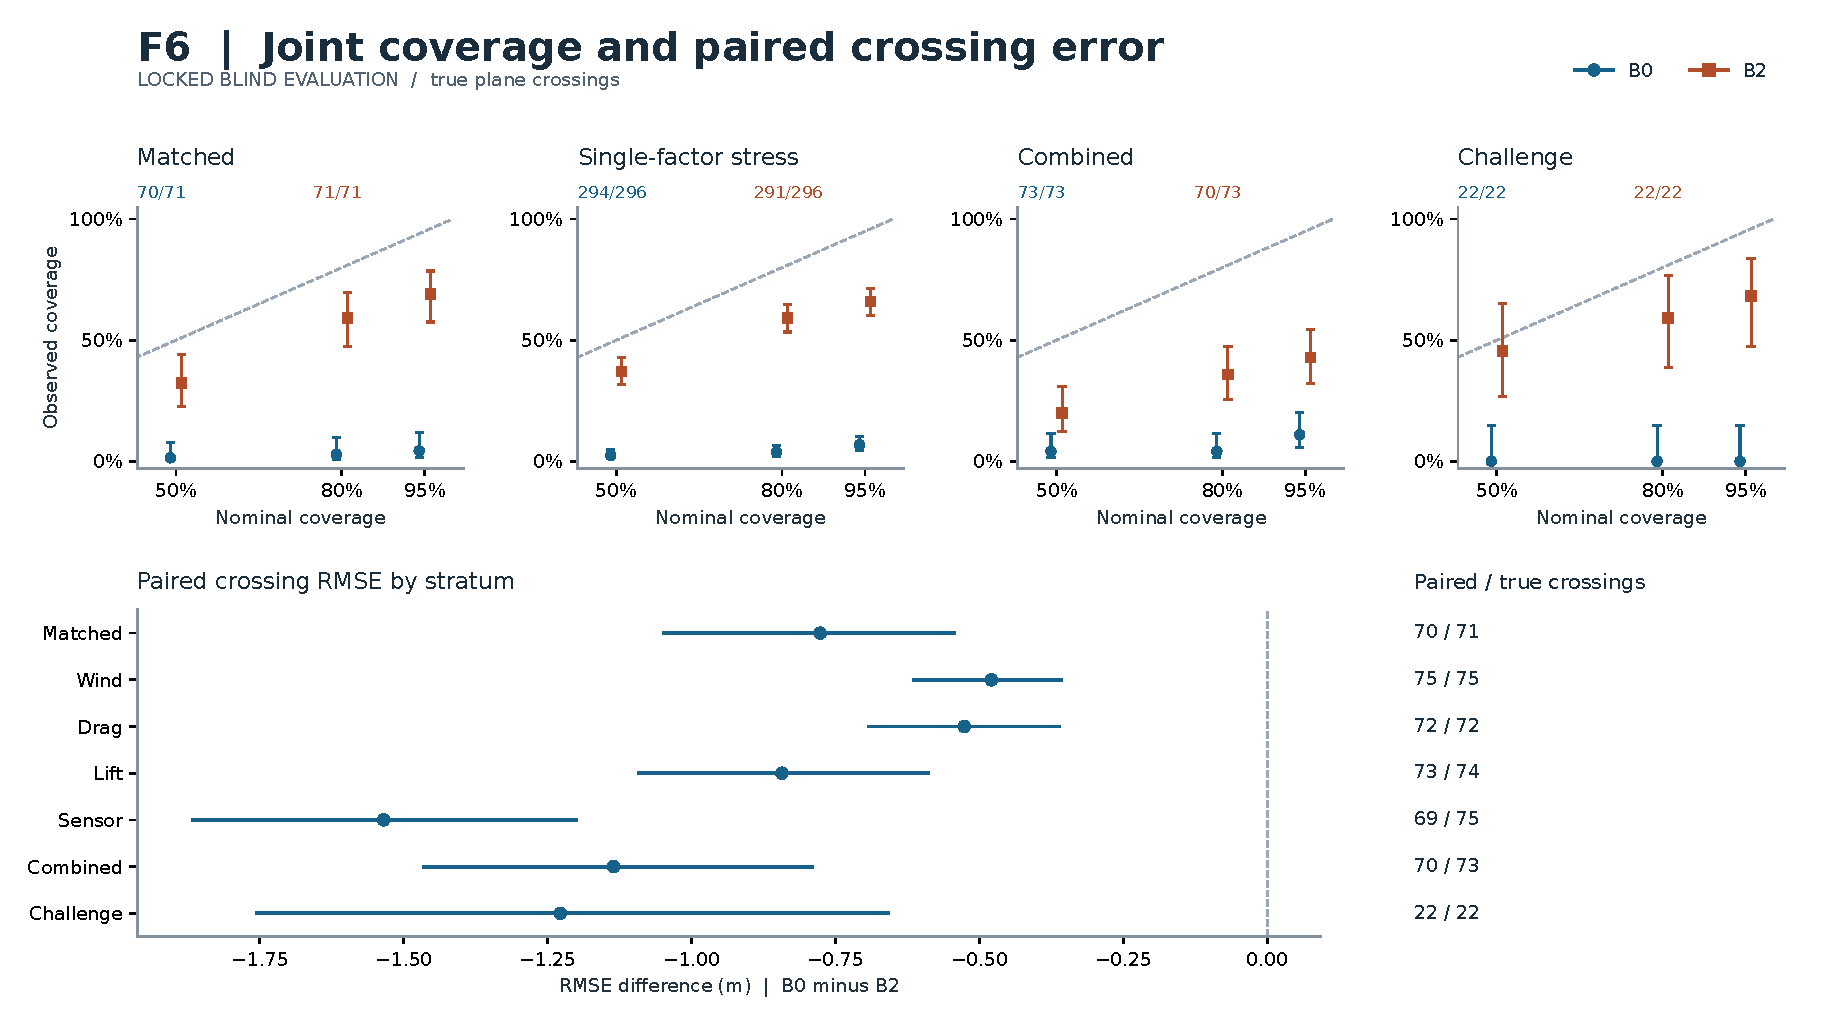
\includegraphics[width=\linewidth]{figures/F6.pdf}
\caption{Joint crossing-region coverage on synthetic trials whose true trajectory crossed the plane. The numerator counts true crossings contained in the highest-mass 0.10 m grid regions. Panel labels show supported forecasts over all true crossings for each model. Vertical bars are 95\% Wilson intervals. Below, selected minus comparator crossing RMSE uses paired conditional-mean forecasts on their common valid cases. Horizontal bars are 95\% percentile intervals from a paired bootstrap within each stratum. Rows below the locked overlap minimum are marked as insufficient.}
\label{fig:F6}
\end{figure}
